\documentclass[a4paper,11pt]{article} 
\usepackage{fancyhdr}
\usepackage{polski}
\usepackage{graphicx}
\usepackage[left=2.5cm,top=2.5cm,right=2.5cm,bottom=4.5cm]{geometry}
\usepackage[T1]{fontenc}
\usepackage{amsfonts}
\usepackage[utf8]{inputenc}
\usepackage{enumerate}
\usepackage{indentfirst}
\usepackage{lipsum}
\usepackage[export]{adjustbox}
\usepackage[font=small,labelfont=bf]{caption} 
\usepackage{booktabs}

\pagestyle{fancy}
\renewcommand{\headrulewidth}{1pt} 
\fancyhead[R]{
\includegraphics[height=80pt]{log.png}
}
\lhead{Akademia Górniczo-Hutnicza \\ im. Stanisława Staszica w Krakowie\\  Wydział Informatyki }
\setlength{\headheight}{80pt}

\cfoot{}
\rfoot{\thepage} 


%%%%%%%%%%%%%%%%%%%%%%%%%DADOS%%%%%%%%%%%%%%%%%%%%%%%%%%%%%
\begin{document}
%\maketitle

%Tabelke umiescic w osobnym pliku
\input{table.txt}

\section{Cel ćwiczenia}
Celem ćwiczenia było wyznaczenie wartości przyspieszenia ziemskiego na podstawie pomiaru okresu drgań wahadła matematycznego oraz wyznaczenie zależności okresu drgań wahadła od jego długości. 
Wahadło matematyczne to ciało o masie punktowej, zawieszone na cienkiej, nieważkiej, nierozciągliwej nici. Wahadło o długości L odchylone o niewielki kąt od pionu i puszczone swobodnie zacznie wykonywać drgania harmoniczne - ich okres T jest dany zależnością $T = 2\pi\sqrt{\frac{L}{g}} $
Wykonując pomiar długości $L$ oraz czasu $T$ można wyznaczyć wartość $g$: $g = \frac{4\pi^2 L}{T^2}$
\section{Potrzebne przyrządy}



\begin{minipage}{10cm}
\vspace{-5cm}
\textbf{Do wykonania ćwiczenia potrzebowaliśmy:}
\begin{itemize}
\item wahadła matematycznego (rysunek obok)
\item linijki
\item stopera
\end{itemize} 
\end{minipage}
\begin{minipage}{5cm}
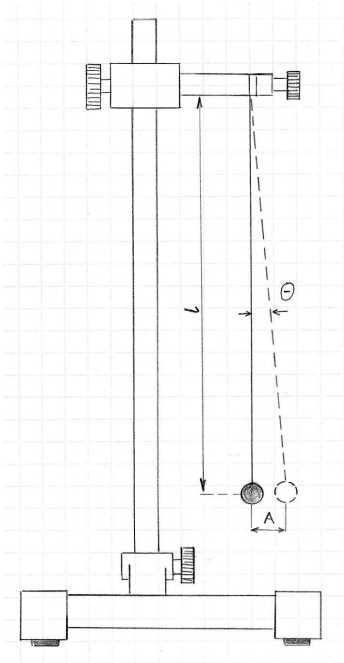
\includegraphics[scale=0.5]{wahadlo.png} 
\end{minipage}

\newpage

\section{Wykonywanie ćwiczenia}
\subsection{Pomiar okresu drgań przy ustalonej długości wahadła}

Długość wahadła $L = 19$ cm, ilość okresów $n=10$

\begin{table}[h]
\centering
\begin{tabular}{|l|l|l|}
\hline
Numer pomiaru & Czas 10 okresów {[}s{]} & Okres T {[}s{]} \\ \hline
1.            & 8,62                    & 0,862                 \\ \hline
2.            & 8,59                    & 0,859                 \\ \hline
3.            & 9,01                    & 0,901                 \\ \hline
4.            & 8,44                    & 0,844                 \\ \hline
5.            & 8,53                    & 0,853                 \\ \hline
6.            & 8,50                    & 0,850                 \\ \hline
7.            & 8,76                    & 0,876                 \\ \hline
8.            & 8,51                    & 0,851                 \\ \hline
9.            & 8,57                    & 0,857                 \\ \hline
10.           & 8,71                    & 0,871                 \\ \hline
\end{tabular}
\end{table}

\noindent \textbf{Niepewność pomiaru okresu:} $$ u(x) = \sqrt{\frac{\displaystyle\sum_{i=1}^{n} (x_i - \overline{x})^2}{n(n-1)}}$$
Gdzie: \\
$n$ - ilość pomiarów \\
$x_i$ - wykonany pomiar \\
$\overline{x}$ - średnia arytmetyczna wszystkich pomiarów

\noindent Zatem dla danych z ćwiczenia mamy:
$$\overline{x} = \frac{0{,}862 +0{,}859 +0{,}901+0{,}844+0{,}853+0{,}85+0{,}876+0{,}851+0{,}857+0{,}871}{10} =0{,}8624 \textrm{ [s]} $$ 
$$ u(x) \stackrel{\textrm{\tiny n=10}}{=} \sqrt{\frac{\displaystyle\sum_{i=1}^{10} (x_i - \overline{x})^2}{10\cdot(10-1)}} = 
\sqrt{\frac{0{,}0025004}{90}}
\approx 5{,}27\cdot 10^{-3}\quad\textrm{[s]}$$

\noindent \textbf{Niepewność pomiaru długości wahadła:}\\
Niepewność pomiaru długości wahadła zależy od urządzenia pomiarowego, jakiego użyliśmy do wykonania ćwiczenia. W naszym przypadku wynosi ona 1 mm.

\vspace{2cm}

\noindent \textbf{Obliczanie wartości przyspieszenia ziemskiego:}\\
Do wyliczenia wartości przyspieszenia ziemskiego użyjemy wzoru na okres dla wahadła matematycznego, którego używaliśmy.
$$T = 2\pi\sqrt{\frac{L}{g}} $$
Po przeszktałceniu otrzymujemy:
$$g = \frac{4\pi^2L}{T^2} $$
Zatem:
$$g = \frac{4\pi^2\cdot 0{,}19 \textrm{ m}}{(0{,}8624 \textrm{ s})^2} \approx 10{,}09\,\frac{\textrm{m}}{\textrm{s}^2}$$

Obliczyliśmy wartość przyspieszenia ziemskiego, teraz należy oszacować niepewność tej wartości. Użyjemy do tego prawa przenoszenia niepewności, co opisuje poniższy wzór:
$$u(g) = \sqrt{\displaystyle \sum_{i=1} ^N \left( \frac{\partial f}{\partial x_i}\right)^2 u^2(x_i)}$$
Dla przyspieszenia ziemskiego przyjmuje on postać:
$$u_c(g) = \sqrt{\left[ \frac{\partial g}{\partial L} \cdot u(L) \right]^2 +\left[ \frac{\partial g}{\partial T} \cdot u(T) \right]^2} $$
Zatem:
$$u_c(g) = \sqrt{\left[ \frac{4\pi^2}{T^2} \cdot u(L) \right]^2 +\left[ \frac{-2\cdot 4\pi^2\cdot L}{T^3} \cdot u(T) \right]^2} $$
\noindent Gdzie: \\
$T = 0{,}8624 $ s\\
$L = 0{,}19 $ m\\
$u(T) = 5{,}27\cdot 10^{-3}\textrm{ s} $ \\
$u(L) = 0{,}001$ m
Po podstawieniu tych wartości do wyżej podanego wzoru otrzymujemy:
$$u_c(g) = \sqrt{\left[ \frac{4\pi^2}{(0{,}8624 \textrm{ s})^2} \cdot 0{,}001 \textrm{ m} \right]^2 +\left[ \frac{-2\cdot 4\pi^2\cdot 0{,}19 \textrm{ m}}{(0{,}8624 \textrm{ s})^3} \cdot  5{,}27\cdot 10^{-3}\textrm{ s} \right]^2} \approx 0{,}13\,\frac{\textrm{m}}{\textrm{s}^2}$$

\noindent Niepewność rozszerzona:
Niepewność rozszerzoną $U_p(g)$ policzymy ze wzoru $U_p(g) = k_p\cdot u_c(g)$, gdzie $k$ jest współczynnikiem rozszerzenia. Przyjmujemy $k_p = 2$. Zatem nasza niepewność rozszerzona jest równa $U_p(g) = 2\cdot u_c(g) = 0{,}26\,\frac{\textrm{m}}{\textrm{s}^2}$

Korzystając z wartości tabelarycznych przyspieszenia ziemskiego dla polskich miast możemy zaobserwować, że uzyskana przez nas wartość równa $g=10{,}09\,\frac{\textrm{m}}{\textrm{s}^2}$ różni się od wartości tabelarycznej dla Krakowa, która wynosi $g=9{,}811\,\frac{\textrm{m}}{\textrm{s}^2}$. Co więcej, niestety nasza wartość nie mieści się w zakresie wyilczonej niepewności rozszerzonej, według której powinniśmy uzyskać wynik z przedziału $\left[9{,}551;10{,}071\right]\, \frac{\textrm{m}}{\textrm{s}^2}$.
\newpage
\subsection{Pomiar zależności okresu drgań od dlugości wahadła}

\begin{table}[h]
\centering
\begin{tabular}{|l|l|l|l|}
\hline
Numer pomiaru & Długość wahadła {[}cm{]} &Czas 10 okresów {[}s{]} & Okres T {[}s{]} \\ \hline
1.            &7,5 & 5,28                    & 0,528                \\ \hline
2.            &11,5 & 6,25                    & 0,625                 \\ \hline
3.            &15,4 & 7,44                    & 0,744                 \\ \hline
4.            &19 & 8,64                    & 0,864                 \\ \hline
5.            &22 & 9,18                    & 0,918                 \\ \hline
6.            &25 & 10,03                    & 1,003                 \\ \hline
7.            &28 & 10,5                    & 1,05                 \\ \hline
8.            &33,5 & 11,28                    & 1,128                 \\ \hline
9.            &40 & 12,37                    & 1,237                 \\ \hline
10.           &52 & 14,12                    & 1,412                 \\ \hline
\end{tabular}
\end{table}
\begin{center}
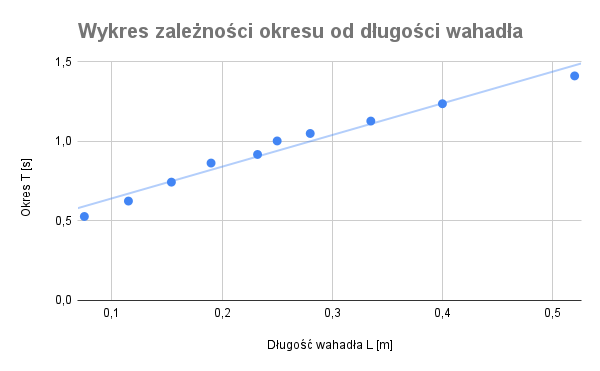
\includegraphics[scale=0.55]{wyk1.png}
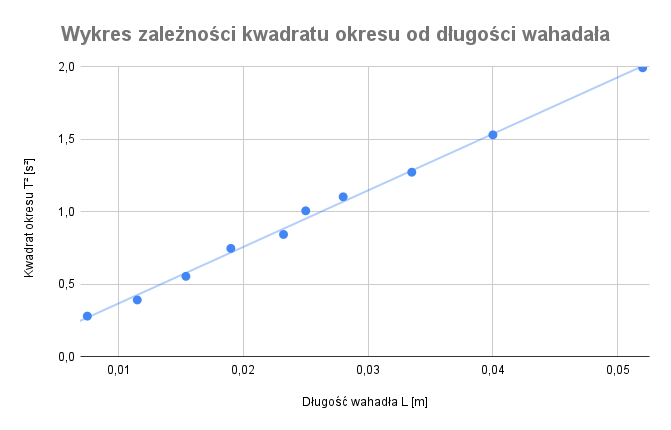
\includegraphics[scale=0.5]{wyk2.png}
\end{center}
Na wykresie zależności kwadratu okresu od długości wahadła linia trendu ma współczynnik kierunkowy równy $3{,}902$. Z zależności $a = \frac{4\pi^2}{g}$ otrzymujemy, że wartość przyspieszenia ziemskiego można policzyć korzystając ze wzoru $g = \frac{4\pi^2}{a}$. Po podstawieniu za zmienną $a$ wartość wyznaczonego wspołczynnika kierunkowego, przyspieszenie ziemskie wyniesie $g = \frac{4\pi^2}{3{,}902} \approx 10{,12}\, \frac{\textrm{m}}{\textrm{s}^2}$

\section{Wnioski}

Uzyskane przez nas wyniki odbiegają od wartości rzeczywistej oraz nie mieszczą się w wyliczonym zakresie niepewności rozszerzonej. Wpływ na to mogło mieć m.in. brak uwzględnienia błędu pomiaru czasu wynikającego z czasu reakcji człowieka oraz wahadło odbiegające od cech wahadła matematycznego.
\end{document}